\documentclass[10pt,final,journal]{IEEEtran}
\usepackage{amsfonts}
\usepackage{amssymb}
\usepackage{graphicx}
\usepackage{siunitx}
\usepackage[dvipsnames]{color}

\title{Feasibility of Harvesting Power To Run A Domestic Water Meter Using Streaming Cell Technology}

\author{Mark~H.~Jones and Jonathan~Scott}

\begin{document}
    \maketitle

    \begin{abstract}
        We investigate the possibility of using streaming cells as a means of harvesting energy from the town water supply.
        We measure the electrical power developed from streaming cells using tap water.
        We estimate the amount of energy available from a typical domestic household based on water usage data.
        We estimate the amount of energy required to operate a simple data logger and transmitter.
        From these estimates we calculate the required efficiency and physical form of a streaming cell energy converter.
        We comment on the feasibility of using streaming cell technology as a means of harvesting energy from a domestic water supply.
    \end{abstract}

    \section{Introduction}
    Domestic and commercial water metering is becoming increasingly common throughout the world.~\cite{Chang2012}
    Cheap and reliable methods of retrieving metered data is an important consideration for utility companies.

    The introduction of wireless automatic meter readers offers many advantages to suppliers of town water.
    These advantages include reduced error rates associated with collecting data, increased billing frequency, leak detection and the elimination of the need for meter readers to access the consumers' property.~\cite{Chang2012,Britton2013}

    The location of a typical water meter means electrical power is usually provided by long life batteries.
    The batteries used in automatic meter readers are non-rechargeable and have a life-span of 10 years.~\cite{BMeters2014}
    The possibility of harvesting energy at the meter should allow frequent data reporting with less maintenance.
    Removing the batteries from current meter reading systems should reduce both the total cost of ownership and electrical waste.

    Streaming cells provide a way of converting fluid energy into electrical energy without moving parts.
    They work on the principle that charged surfaces in contact with ionic solutions attract counter-ions so as to form a charged layer at the contact surface.~\cite{Stein2004}
    This charged layer is termed the double layer and is the key mechanism that enables streaming cell energy conversion.
    The conversion is made by forcing ions within the double layer through narrow channels with the application of hydrostatic pressure.

    \begin{figure}
        \begin{center}
        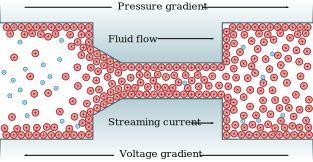
\includegraphics{diagram_streamingCellPrinciple}
        \end{center}
        \caption{Conceptualised rendering of the cross section of a streaming cell.
        Positive ions are being forced through the cavity by the application of pressure.}
        \label{fig:streamingPrinciple}
    \end{figure}

    A double layer is called such because it is made of two individual layers; the Stern and diffuse layers.
    The Stern layer is comprised of immobilised ions at the charged solid surface.~\cite{Salieb-Beugelaar2009}
    The diffuse layer surrounds the Stern layer and contains counter-ions that are not so strongly bound as to be immobile.
    The thickness of the double layer is defined as the Debye length ($l_{D}$) and is dependant upon the ionic concentration of the liquid.~\cite{Israelachvili2011}
    When the dimensions of a channel become small enough, double layers will overlap.
    Overlapping double layers mean that any co-ions are repelled from within the channel.

    The channels can be created individually using a range fabrication methods, such as chemical etching or the use of narrowly separated parallel plates.
    Channels can also be formed en-mass by using porous materials such as glass or ceramics as the cell where the pores themselves form channels.
    Glass has the attractive property that it obtains a negative surface charge when in contact with water.
    This surface charge is caused by the deprotonation of surface silanol groups in glass (SiOH~$\leftrightarrows$~SiO$^{-}+$~H$^{+}$).~\cite{Kirby2004a}
    By immersing a glass channel in an electrolyte solution, double layers of positive ions (counter-ions in this case) occupy the interior walls of the channel.

    Counter-ions within a streaming cell are transported by applying a pressure gradient across the channel/cell.
    Pressure forces the counter-ion rich fluid through the channel creating a streaming current.
    Streaming currents establish a voltage across the cell, termed streaming potential, due to ionic concentrations at each end of the channel becoming unbalanced.

    Streaming currents have been heavily investigated as a means of generating electrical energy from pressure gradients.~\cite{Chang2009,Daiguji2006,Daiguji2004b,Davidson2008a,Davidson2008,CherngHon2012,Jiao2014,Lu2006,Olthuis2005,Osterle1964,Pennathur2007,Ren2008a,VanderHeyden2006,Heyden2007,Xie2008,Yang2003}
    Theoretical predictions of the efficiency of standard micro/nano-fluidic channels are 2\% for pure water and 7\% for sodium chloride.~\cite{VanderHeyden2006}
    Experimental results show conversion efficiencies in the range of:
    \begin{itemize}
        \item 0.01\% by forcing water through porous glass with pore sizes from 10\thinspace--\SI{16}{\micro\metre}.~\cite{Yang2003}
        \item 0.8\% by forcing pure water through a ceramic rod populated with \SI{6}{\micro\metre} pores.~\cite{Yang2004}
        \item 3\% by forcing sodium chloride solution through a \SI{75}{\nano\metre} by \SI{50}{\micro\metre} silica channel.~\cite{Heyden2007}
        \item 0.77\% by forcing sodium chloride through a \SI{200}{\nano\metre} pore in an alumina membrane.~\cite{Lu2006}
        \item 5\% by forcing sodium chloride solution through a \SI{0.5}{\nano\metre} cylindrical pore in polyethylene terephalate foil.~\cite{Xie2008}
    \end{itemize}
    These results indicate that small channels using solutions containing salt are more efficient.
    According to \cite{Daiguji2004b}, the efficiency is maximised when the channel height is about half the Debye length.
    For water with a sodium content in the range 1--100~ppm this equates to a channel height in the order of 100--10~nm.
    Additionally, ~\cite{VanderHeyden2006} states that the maximum efficiency is found when the salt concentration is low.


    It is clear from the literature that there is significant progress to be made with respect to increasing the conversion efficiency.
    Techniques to induce hydrodynamic slip at the fluid-solid interface are predicted to increase this efficiency to 30-40\%.~\cite{Davidson2008a, Ren2008a}
    Experimental results utilising slip enhanced channels have not yet been reported in the literature.
    This type of enhancement would overcome the `no-slip boundary condition' at the solid-liquid interface.
    Slip at the interface boundary would mean that ions in the Stern layer, where ionic concentration is highest, could also be moved through the channel.
    Surface enhanced channels are out of the scope of this study due to cost and manufacturing difficulty.

    We address the question of whether it is feasible to build a harvester using readily available materials.
    Such a harvester must produce enough energy to operate a microprocessor and radio communication device.
    It must collect all of its energy from a domestic water supply and be reliable.

    The remainder of this work is presented as follows.
    In section \ref{sect:streamingCell} we build, measure and calculate the conversion efficiency of a simple streaming potential cell.
    We confirm the relationship between pressure and applied pressure and investigate the effect of channel height.
    In section \ref{sect:waterConsumption} we estimate the amount of harvestable energy from a domestic water usage profile.
    Section \ref{sect:powerRequirements} quantifies energy requirements of a simple electronic meter.
    And finally, we conclude with a discussion on the feasibility of using streaming cells to harvest energy.

    \section{Readily Attainable Streaming Cell Efficiency} \label{sect:streamingCell}
    \begin{figure}
        \begin{center}
        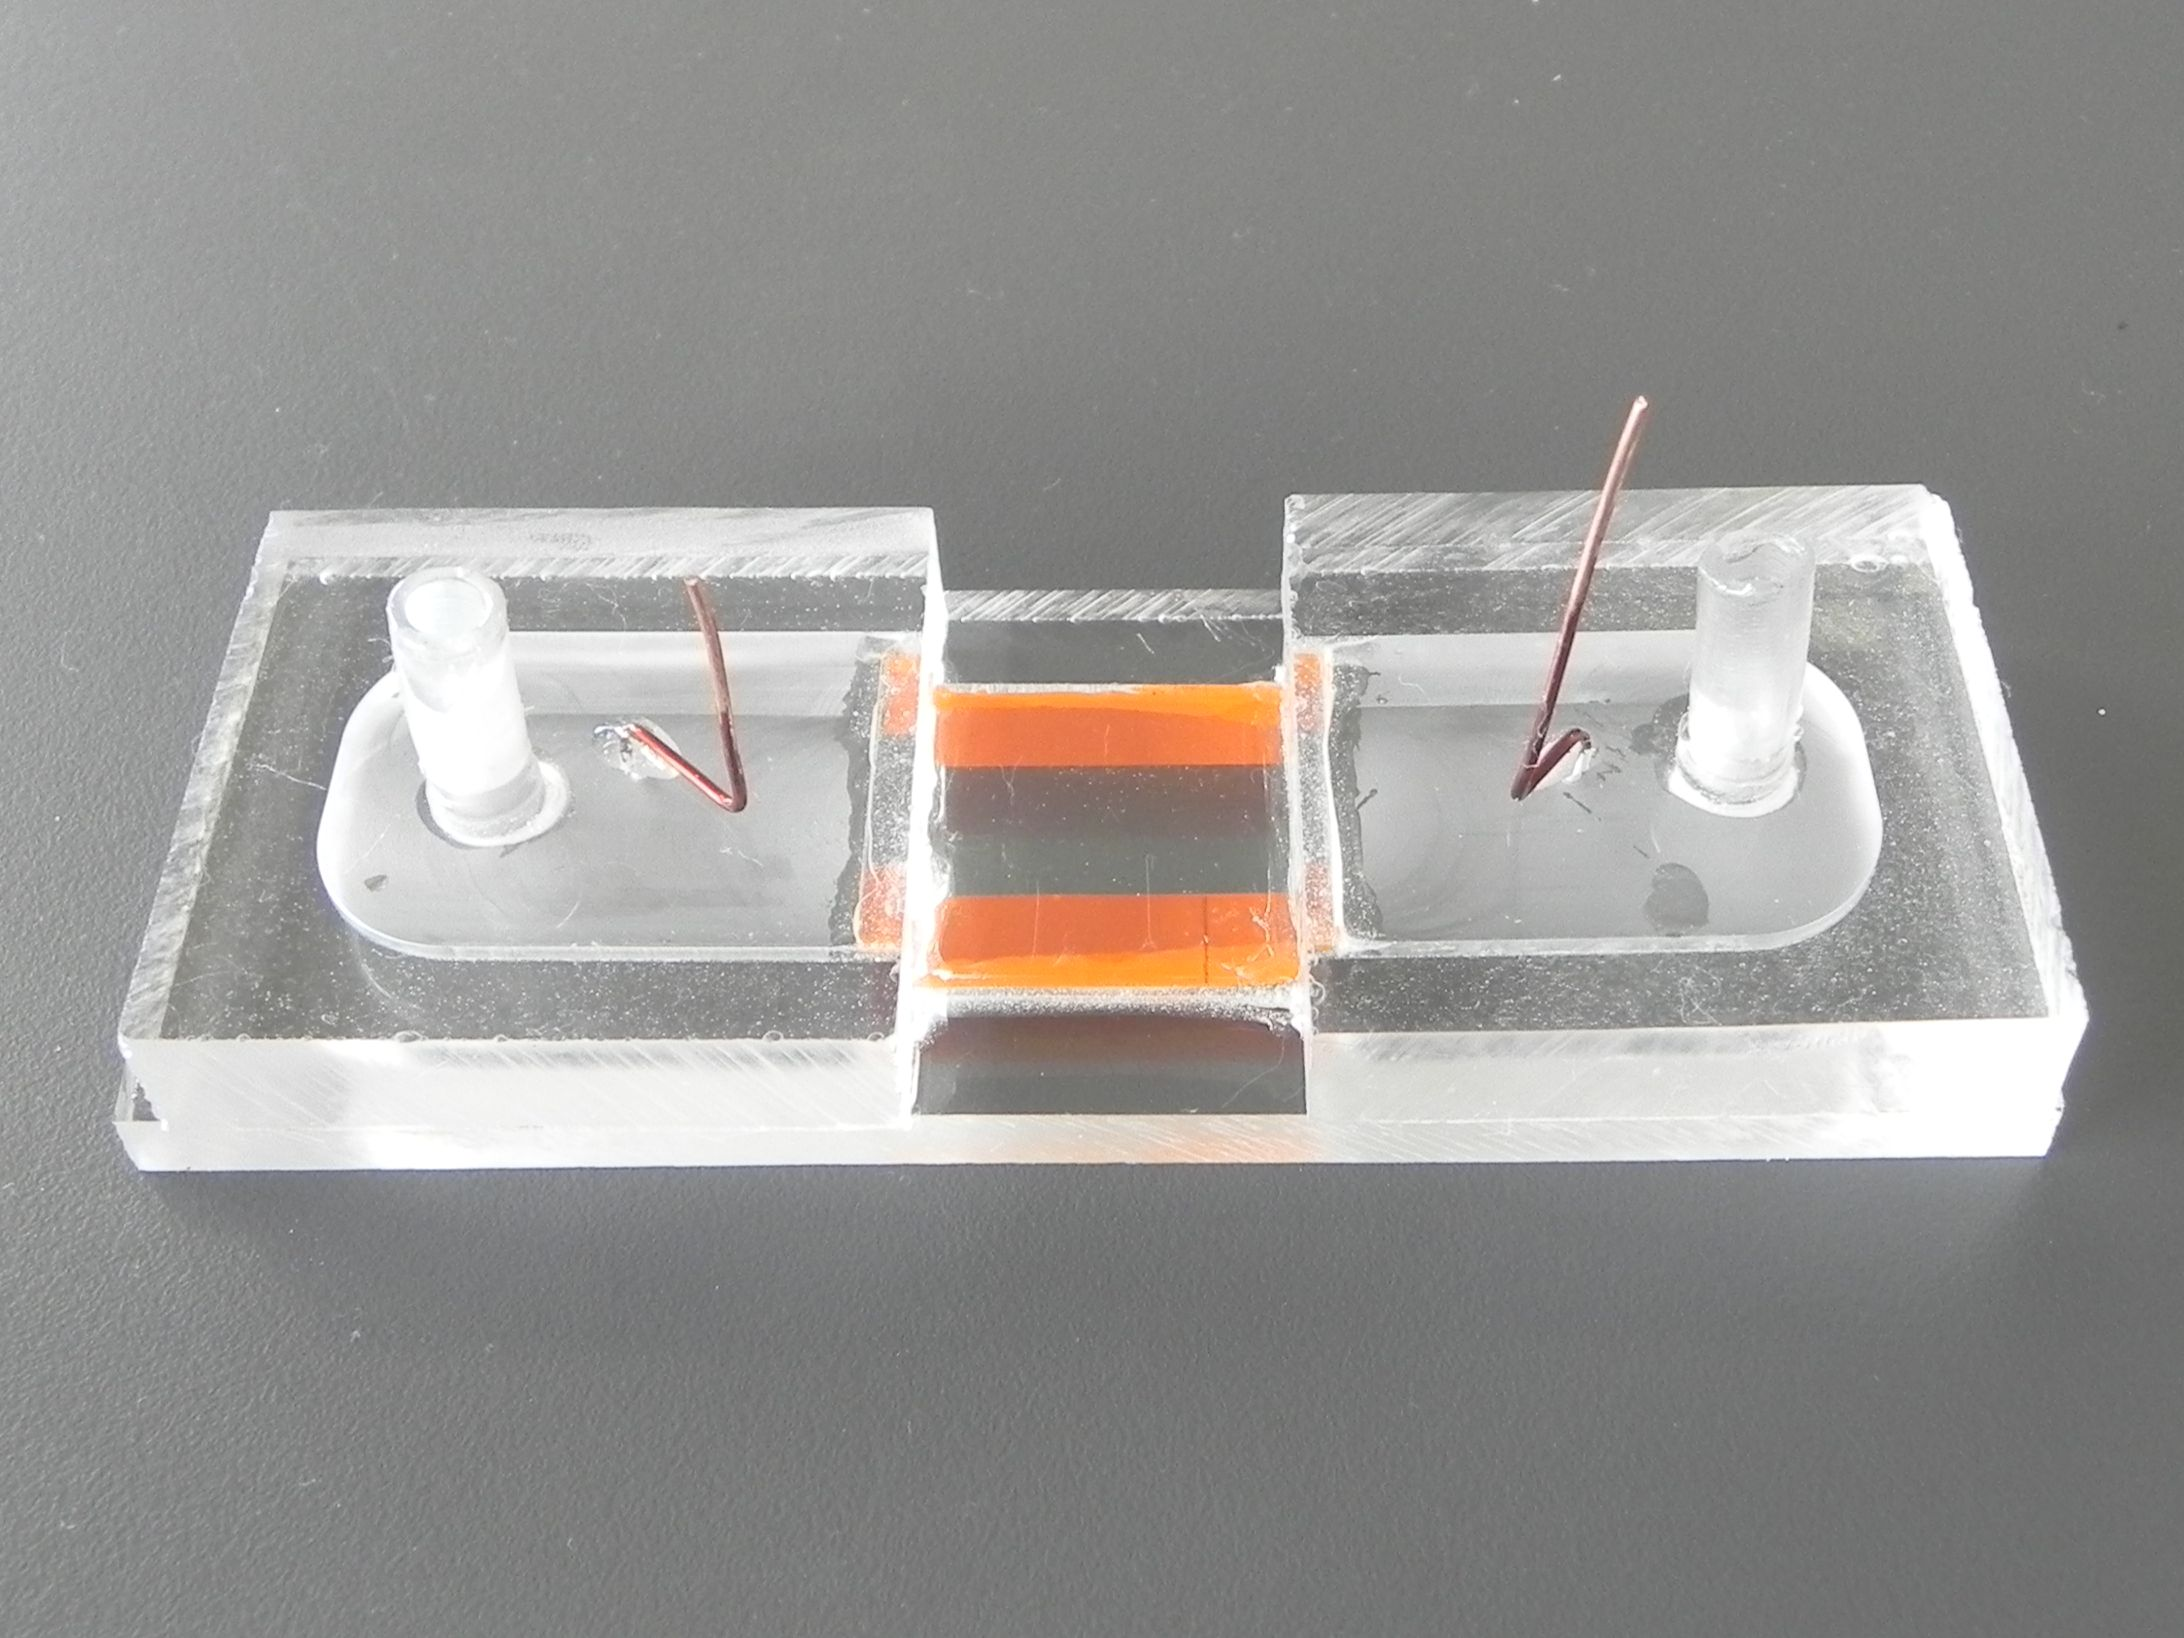
\includegraphics[width=\linewidth]{Photo_streamingPotential_Assembly_Step3.JPG}
        \end{center}
        \caption{One of our ten constructed streaming cells mounted in an acrylic holder. Copper wires have been epoxied into each side to provide a means of measuring the developed potential across the cell. The plastic shims are visible as the orange strips at each side of the cell.}
        \label{fig:cell}
    \end{figure}

    In~\cite{Gu2000}, the authors employ a relatively simple parallel plate design to create a streaming cell.
    They glued plastic shims between parallel plates of glass, providing a simple way of setting a channel's height.
    Using that method, the authors fabricated three cells with channel heights of \SI{50}{\micro\metre}, \SI{100}{\micro\metre} and \SI{150}{\micro\metre}.
    Each of the channels were \SI{3}{\centi\metre} long and had a inner width of \SI{1}{\centi\metre}.

    We replicate the approximate dimensions of \cite{Gu2000} to produce ten streaming cells.
    The approximate internal channel heights of these channels are \SI{245}{\micro\meter}, \SI{178}{\micro\meter}, \SI{161}{\micro\meter}, \SI{125}{\micro\meter}, \SI{106}{\micro\meter}, \SI{75}{\micro\meter}, \SI{71}{\micro\meter}, \SI{56}{\micro\meter}, \SI{52}{\micro\meter}, and \SI{26}{\micro\meter}.
    The channels are made from glass microscope slides (Sail Brand - JIA 7101WT) sectioned into halves.
    Plastic shims (Garlock Colorplast) are epoxied (Selleys Araldite Ultra Clear Resin) between slide halves to separate the slides.
    The dimensions at each end of each channel are measured under a microscope to determine the channel height once the channels had set.

    Each channel is epoxied between two acrylic reservoirs and a base plate.
    This provides a rigid structure under pressure and provides connection of wires and hoses.
    Copper wires and silicon hoses are inserted into each reservoir to facilitate voltage measurement and the application of pressure.
    A photo of one of the cells is shown in Fig. \ref{fig:cell}.

    Pressure is applied to the cell by connection to tap and leaving the output connection open to atmosphere.
    A Honeywell pressure sensor (model 26PC15SMT) is placed across the cell to measure applied pressure.
    An Agilent precision measurement mainframe (model E5270B) is used to measure streaming potential, streaming current and to read the pressure sensor's output.
    The working fluid, being tap water, had a conductivity of \SI{183e-6}{\siemens\per\meter} as measured with an EDT Instruments RE 388Tx Conductivity Meter.

    Measured pressure-to-voltage gradients from each of the ten streaming cells are presented in Fig.~\ref{fig:cellEfficiency}.
    Spread in the data is attributed to uncertainty in the internal dimensions of each cell.
    Due to the opacity of the resin used, measurement of the internal cell dimensions was not possible.
    The plot shows the relationship between channel height and voltage gradient per Pascal of applied pressure.
    Each cell had a different flow rate, which this plot does not take into account.
    Three of the cells burst before flow measurements were obtained.
    % The \SI{26}{\micro\meter} channel shows a much lower gradient due to . which we expect is a result of a reduced flow rate.
    % The \SI{26}{\micro\meter} cell burst before we obtained flow rate measurements.

    \begin{figure}
        \begin{center}
        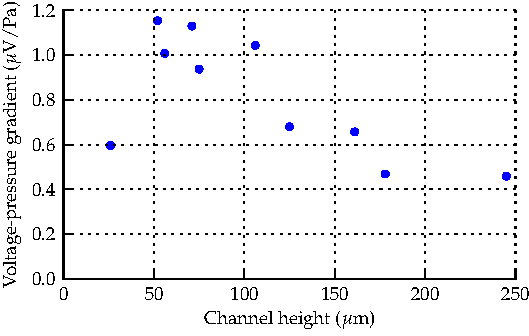
\includegraphics[width=\linewidth]{graph_cellEfficiency}
        \end{center}
        \caption{Gradient of developed streaming voltage with applied pressure differential versus the channel height of ten fabricated streaming cells.}
        \label{fig:cellEfficiency}
    \end{figure}

    \begin{figure}
        \begin{center}
        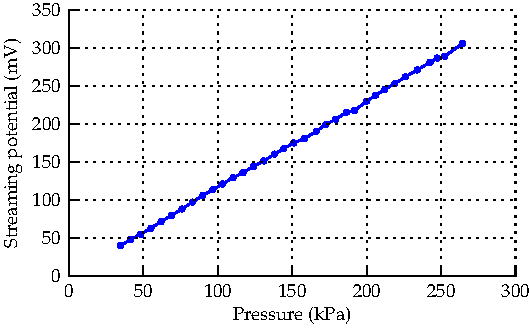
\includegraphics[width=\linewidth]{graph_voltagePressure}
        \end{center}
        \caption{Measured voltage developed across the \SI{52}{\micro\meter} streaming cell as a function of the differential pressure across the cell.}
        \label{fig:cellVoltagePressure}
    \end{figure}

    We now measure available power output of the \SI{71}{\micro\meter} streaming cell.
    This cell was chosen as it remained mechanically robust and had good output characteristics.
    We measure the streaming voltage and pressure while sweeping the electrical current draw from the device.
    The applied pressure was held at \SI{260}{\kilo\pascal} for the duration of the measurement and the flow rate was previously determined to be \SI{2.05}{\milli\litre\per\second}.

    Fig.~\ref{fig:cellOutput} shows the measured data along with the calculated power curve.
    Using the power curve we calculate the cell's internal electrical resistance to be \SI{5.6}{\mega\ohm}.
    Peak output power of \SI{1.52}{\nano\watt} is delivered when the current draw is \SI{33.5}{\nano\ampere} with a voltage of \SI{182}{\milli\volt}.

    Based on the pressure applied and the flow rate through the cell, the input power is \SI{539}{\milli\watt}.
    Energy conversion efficiency is in the order of $1\times 10^{-6}\%$.

    \begin{figure}
        \begin{center}
        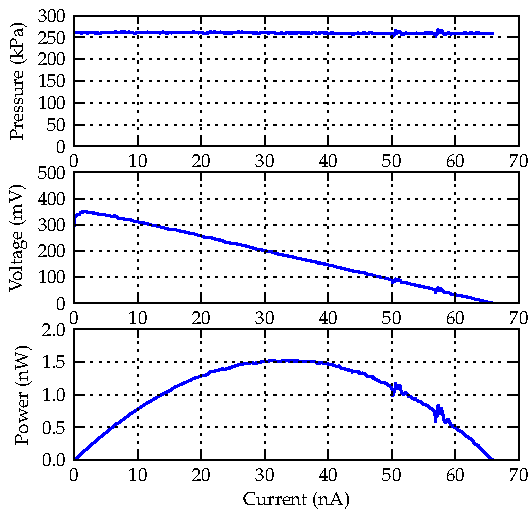
\includegraphics[width=\linewidth]{graph_cellOutput}
        \end{center}
        \caption{Streaming cell output voltage as a function of drawn current with constant pressure.
        The cell's calculated output power appears in the lower plot with a peak at approximately \SI{33.5}{\nano\ampere}.}
        \label{fig:cellOutput}
    \end{figure}


    % Based on measurements of the \SI{52i}{\micro\meter} channel we estimate the amount of electrical power available for harvesting.
    % Fig.~\ref{fig:equivalentCircuit} shows the equivalent circuit for a streaming potential cell delivering a streaming current ($I_{S}$).
    % The the streaming potential ($V_{S}$) was measured with no load resistance ($R_{L}$) due to the use of the E5270 preventing load current being drawn.
    % The dimensions of the cell together with the conductivity of the working fluid give the cell an internal resistance ($R_{ch}$) of approximately \SI{30}{\giga\ohm}.
    % Using these parameters, the available output power from the cell has been calculated and is presented in Fig.~\ref{fig:cellPowerPressure} with respect to the applied pressure.



    % \begin{figure}
    %     \begin{center}
    %     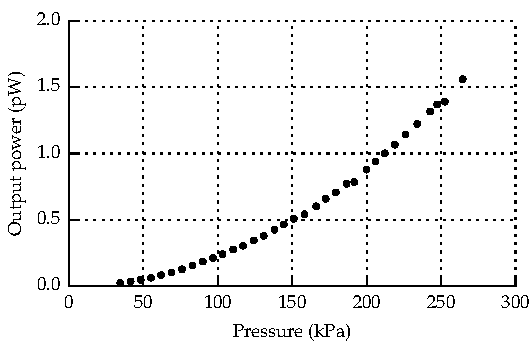
\includegraphics[width=\linewidth]{graph_powerPressure}
    %     \end{center}
    %     \caption{Maximum power available to an external load placed across the \SI{52}{\micro\meter} cell as a function of pressure differential. Power has been calculated using a load resistance of \SI{30}{\giga\ohm} where only half of total power is available to the load. Note that the units of power are expressed in picoWatts.}
    %     \label{fig:cellPowerPressure}
    % \end{figure}


    \section{Estimation of Harvestable Energy From A Typical New Zealand Dwelling}
    \label{sect:waterConsumption}

    % \begin{figure}
    %     \begin{center}
    %     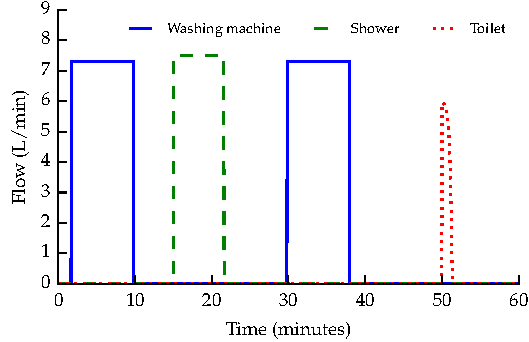
\includegraphics[width=\linewidth]{graph_profile}
    %     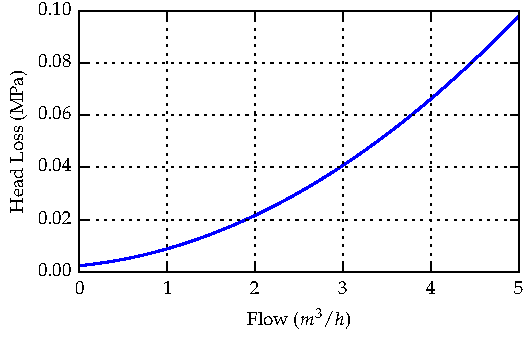
\includegraphics[width=\linewidth]{graph_pressureLoss}
    %     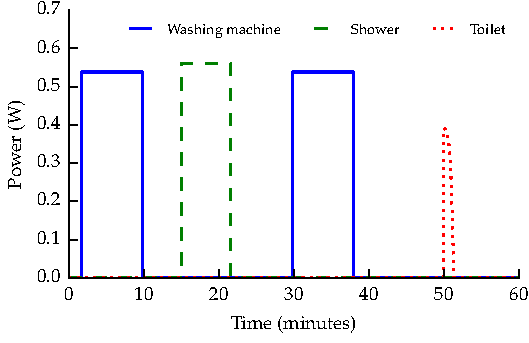
\includegraphics[width=\linewidth]{graph_harvest}
    %     \end{center}
    %     \caption{
    %     Calculation of the power dissipation inside a typical water meter.
    %     The top figure shows flow profiles for one washing machine use, a shower and a toilet flush in a typical dwelling.
    %     Underneath is the head loss curve from a typical domestic water meter as a function of flow rate.
    %     The lower figure presents each of the water usage events (shower, washing machine and toilet flush) in terms of power dissipated inside the water meter due to mechanical losses.
    %     Dissipated power is calculated from the head loss curve and the flow rate data of the upper graphs.
    %     }
    %     \label{fig:profileSample}
    % \end{figure}

    \begin{figure}
        \begin{center}
        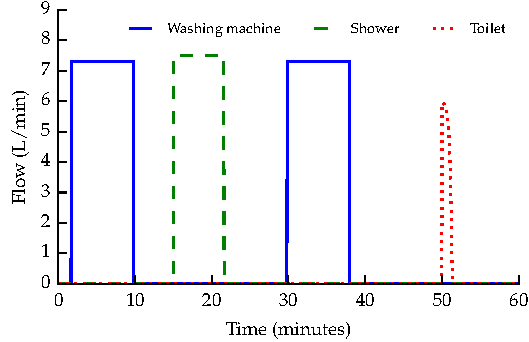
\includegraphics[width=\linewidth]{graph_profile}
        \end{center}
        \caption{Sample profile showing constructed instances of washing machine use, a shower and a toilet flush.
        Washing machine usage is broken into two parts corresponding to a wash and rinse cycle.}
        \label{fig:profileSample}
    \end{figure}

    \begin{figure}
        \begin{center}
        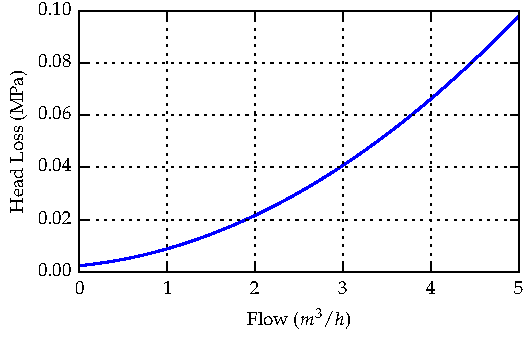
\includegraphics[width=\linewidth]{graph_pressureLoss}
        \end{center}
        \caption{Estimated head loss from a mechanical water meter typically installed in a domestic setting.}
        \label{fig:headloss}
    \end{figure}

    \begin{figure}
        \begin{center}
        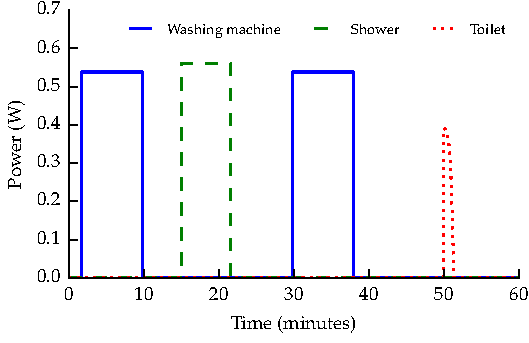
\includegraphics[width=\linewidth]{graph_harvest}
        \end{center}
        \caption{Calculated power dissipation by a typical domestic mechanical water meter for each of the sample profile events.}
        \label{fig:powerDissipated_meter}
    \end{figure}


    In \cite{Heinrich2008} the authors monitor water consumption of 51 homes throughout Auckland, New Zealand between February and September of 2008.
    The report shows that the majority of domestic water is consumed by the shower (30\%), washing machine (27\%) and toilet (20\%).
    Together these account for over three quarters of the indoor water usage in the average home.
    We have created a flow profile from which to calculate the available harvestable energy using data from both \cite{Heinrich2008} and \cite{Heinrich2007}.
    The profile fits the usage statistics of a home with two occupants according to the previously mentioned reports over the duration of a week.
    The during that time five uses of a washing machine, fourteen showers and fifty six toilet flushes occur.
    A sample of the usage profiles of each item is shown in Fig. \ref{fig:profileSample}.

    Figure~\ref{fig:headloss} shows the pressure head loss curve from a water meter typically installed at New Zealand homes (Kent PSMT 25mm).~\cite{WatercareNewZealand2014}
    Using this curve we calculate power dissipation in a water meter during a washing machine cycle, shower, and toilet flush; presented as Fig.~\ref{fig:powerDissipated_meter}
    The total energy dissipated within the meter for each events is:
    \begin{itemize}
    \item \SI{547}{\joule} per load of washing,
    \item \SI{222}{\joule} per shower, and
    \item \SI{24.3}{\joule} per flush of the toilet.
    \end{itemize}

    % These figures are based on average duration and flow rates as found in \cite{Heinrich2008}, and the estimated head loss from Fig.~\ref{fig:headloss}.
    Over an average week the the reference water meter would dissipate approximately \SI{7.20}{\kilo\joule} of energy; averaging \SI{1.03}{\kilo\joule} per day.

    \section{Estimation of Energy Requirements}
    \label{sect:powerRequirements}
    In \cite{Jones2011} we measure the energy efficiency of various low-power microcontrollers.
    Here we take measured data from that paper to estimate a smart meter's energy requirements.
    Measurements of an Atmel ATtiny 25V have been used as it offered good performance over a wide range of processor functions.
    A crude estimation of the processor's event loop is as follows:
    \begin{itemize}
    \item Sleep for \SI{1}{\second} (\SI{97.4}{\nano\joule})
    \item Execute 1 000 instructions (\SI{1.14}{\micro\joule})
    \item Take 2 ADC measurements (\SI{2.56}{\nano\joule})
    \item Write 2 bytes to non-volatile memory (\SI{79.0}{\micro\joule})
    \end{itemize}
    Every six hours the device will transmit metered data by doing the following actions:
    \begin{itemize}
    \item Execute 1 000 000 instructions (\SI{1.14}{\milli\joule})
    \item Transmit 100 bytes of data over zigbee radio (\SI{12.3}{\milli\joule})
    \item Write 10 bytes to non-volatile memory (\SI{394}{\micro\joule})
    \end{itemize}

    The energy requirements for a 100 byte data transmission over ZigBee (Digi International XBee S2) is presented as Fig.~\ref{fig:xbeePower} (recorded using a Tektronix TDC 2012 Digital Storage Oscilloscope across a \SI{10.2}{\ohm} current sense resistor).

    Our estimation shows a monitoring and transmitting device would need about \SI{6.96}{\joule} per day to operate in ideal transmission conditions.
    If the transmitter were to require $100\times$ more energy to transmit, as an estimate of poor conditions, the energy requirements would jump to \SI{9.39}{\joule} per day.
    It is therefore estimated that an energy harvester would need to deliver approximately \SI{10}{\joule} of energy per day.

    \begin{figure}
        \begin{center}
        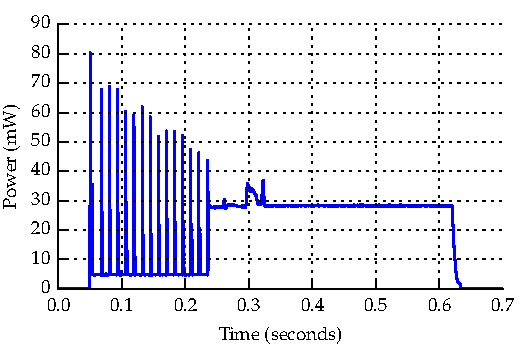
\includegraphics[width=\linewidth]{graph_XbeePower_reduced}
        \end{center}
        \caption{Power draw from a ZigBee wireless module transmitting to a nearby receiver in optimal conditions. The ZigBee module is operated with a 3.3V supply voltage and is powered down between transmissions. The energy required to power-up the ZigBee module and transmit 100 bytes of data is \SI{12.3}{\milli\joule}.}
        \label{fig:xbeePower}
    \end{figure}

    % \section{Estimation of Streaming Cell Harvester}
    % \label{sect:harvesterSize}

    \section{Conclusion}
    \label{sect:conclusion}
    We have calculated approximately \SI{1}{\kilo\joule} of energy is dissipated per day inside a typical water meter at a two occupant dwelling.
    We have estimated that a harvester would need to harvest approximately \SI{10}{\joule} of energy per day to record and transmit water consumption data.
    Therefore an energy harvester with an energy conversion efficiency of 1\% is required.
    Streaming cells we constructed produced conversion efficiencies in the order of $1\times 10^{-6}\%$.

    % \section{Conclusion}
    \bibliographystyle{plain}
    \bibliography{library}

\end{document}
